% -----------------------------------------------------------------------------
%                                     HEADER                                    
% -----------------------------------------------------------------------------
\documentclass[a4paper, 10pt]{article}
\usepackage{jheppub}
\usepackage[T1]{fontenc}
\usepackage{colortbl,xcolor,float}
\definecolor{orange}{rgb}{1,0.5,0}
% -----------------------------------------------------------------------------
%                                   COVER PAGE                                  
% -----------------------------------------------------------------------------
\title{{
\includegraphics[scale=.4]{logo.png}}\ The LaTeX report}

\author{Generated by jaco on 03 November 2020, 12:39:33}

\abstract{
  This report has been generated automatically
  by {\sc MadAnalysis} 5.\\$~$\\ 
  Please cite:\\ 
  \begin{quote}
    \textbf{E.~Conte, B.~Fuks and G.~Serret},\\ 
    \textit{MadAnalysis 5, A User-Friendly
    Framework for Collider Phenomenology},\\ 
    Comput. Phys. Commun. {\bf 184} (2013) 222-256,\\
    arXiv:1206.1599 [hep-ph].\\ 
  \end{quote}
  To contact us:\\ 
  \begin{quote}
    \textbf{http://madanalysis.irmp.ucl.ac.be}\\
    \textbf{ma5team@iphc.cnrs.fr}\\
  \end{quote}
}

% -----------------------------------------------------------------------------
%                                 BEGIN DOCUMENT                                
% -----------------------------------------------------------------------------
\begin{document}
\maketitle
\flushbottom

% -----------------------------------------------------------------------------
%                                 SECTION Setup                                 
% -----------------------------------------------------------------------------
\newpage
\section{ Setup}

\subsection{ Command history}

\texttt{ma5>import /\-home/\-jaco/\-Documents/\-ML4EFT/\-code/\-MG5\_aMC\_v2.8.2/\-MG5\_aMC\_v2\_8\_2/\-bin/\-eft\_benchmark/\-bin/\-internal/\-ufomodel\\
}
\texttt{ }\texttt{ }\texttt{ma5>import /\-home/\-jaco/\-Documents/\-ML4EFT/\-code/\-MG5\_aMC\_v2.8.2/\-MG5\_aMC\_v2\_8\_2/\-bin/\-eft\_benchmark/\-Events/\-run\_03/\-unweighted\_events.lhe.gz as unweighted\_events\\
}
\texttt{ }\texttt{ }\texttt{ma5>define vl = 12 14 16\\
}
\texttt{ }\texttt{ }\texttt{ma5>define vl~ = -16 -14 -12\\
}
\texttt{ }\texttt{ }\texttt{ma5>define invisible = ve ve~ vm vm~ vt vt~ vl vl~\\
}
\texttt{ }\texttt{ }\texttt{ma5>set main.graphic\_render = matplotlib\\
}
\texttt{ }\texttt{ }\texttt{ma5>plot THT   40 0 500 [logY]\\
}
\texttt{ }\texttt{ }\texttt{ma5>plot MET   40 0 500 [logY]\\
}
\texttt{ }\texttt{ }\texttt{ma5>plot SQRTS 40 0 500 [logY]\\
}
\texttt{ }\texttt{ }\texttt{ma5>plot  PT(t~[1]) 40 0  500 [logY]\\
}
\texttt{ }\texttt{ }\texttt{ma5>plot ETA(t~[1]) 40 -10 10 [logY]\\
}
\texttt{ }\texttt{ }\texttt{ma5>plot  PT(t[1]) 40 0  500 [logY]\\
}
\texttt{ }\texttt{ }\texttt{ma5>plot ETA(t[1]) 40 -10 10 [logY]\\
}
\texttt{ }\texttt{ }\texttt{ma5>plot M(t~[1] t[1]) 40 0  500 [logY ]\\
}
\texttt{ }\texttt{ }\texttt{ma5>plot DELTAR(t~[1],t[1]) 40 0 10 [logY ]\\
}
\texttt{ }\texttt{ }\texttt{ma5>submit /\-home/\-jaco/\-Documents/\-ML4EFT/\-code/\-MG5\_aMC\_v2.8.2/\-MG5\_aMC\_v2\_8\_2/\-bin/\-eft\_benchmark/\-MA5\_PARTON\_ANALYSIS\_analysis1\\
}
\texttt{ }\texttt{ }\subsection{ Configuration}

\begin{itemize}
  \item MadAnalysis version 1.8.45 (2020/\-05/\-01).
   \item Histograms given for an integrated luminosity of \textcolor{blue}{10}\textcolor{blue}{ fb}$^{\textcolor{blue}{-1}}$\textcolor{blue}{.}
\textcolor{blue}{}
\end{itemize}
% -----------------------------------------------------------------------------
%                                SECTION Datasets                               
% -----------------------------------------------------------------------------
\newpage
\section{ Datasets}

\subsection{ unweighted\_events}

\begin{itemize}
  \item Sample consisting of: \textcolor{blue}{signal}  events.
   \item Generated events: \textcolor{blue}{10000 }  events.
   \item Normalization to the luminosity: \textcolor{blue}{-1314}\textcolor{blue}{ +/\-- }\textcolor{blue}{3 }  events.
   \item Ratio (event weight): \textcolor{blue}{-0.13 } .  
 
\end{itemize}
\begin{table}[H]
  \begin{center}
    \begin{tabular}{|m{55.0mm}|m{25.0mm}|m{30.0mm}|m{30.0mm}|}
      \hline
      {\cellcolor{yellow}         Path to the event file}& {\cellcolor{yellow}         Nr. of events}& {\cellcolor{yellow}         Cross section (pb)}& {\cellcolor{yellow}         Negative wgts (\%)}\\
      \hline
      {\cellcolor{white}          eft\_benchmark/\-Events/\-run\_03/\-unweighted\_events.lhe.gz}& {\cellcolor{white}          10000}& {\cellcolor{white}          -0.131 @ -0.19\%}& {\cellcolor{white}          99}\\
\hline
    \end{tabular}
  \end{center}
\end{table}

% -----------------------------------------------------------------------------
%                            SECTION Histos and cuts                            
% -----------------------------------------------------------------------------
\newpage
\section{ Histos and cuts}

\subsection{ Histogram 1}

\textbf{* Plot: THT}\\
   \begin{table}[H]
  \begin{center}
    \begin{tabular}{|m{23.0mm}|m{23.0mm}|m{18.0mm}|m{19.0mm}|m{19.0mm}|m{19.0mm}|m{19.0mm}|}
      \hline
      {\cellcolor{yellow}         Dataset}& {\cellcolor{yellow}         Integral}& {\cellcolor{yellow}         Entries per event}& {\cellcolor{yellow}         Mean}& {\cellcolor{yellow}         RMS}& {\cellcolor{yellow}         \% underflow}& {\cellcolor{yellow}         \% overflow}\\
      \hline
      {\cellcolor{white}         unweighted\_events}& {\cellcolor{white}         0.0 +/\-- 0.0}& {\cellcolor{white}         1.0}& {\cellcolor{white}         0.0}& {\cellcolor{white}         0.0}& {\cellcolor{green}         0.0}& {\cellcolor{green}         0.0}\\
\hline
    \end{tabular}
  \end{center}
\end{table}

\begin{table}[H]
  \begin{center}
    \begin{tabular}{|m{140.0mm}|}
      \hline
      {\cellcolor{white}\textcolor{red}{Warnings related to negative event-weights:}}\\
      \hline
      {\cellcolor{white}\textcolor{red}{dataset=unweighted\_events -> bin 0 has a negative content : -1314.515. This value is set to zero}}\\
      \hline
\hline
    \end{tabular}
  \end{center}
\end{table}

\begin{figure}[H]
  \begin{center}
    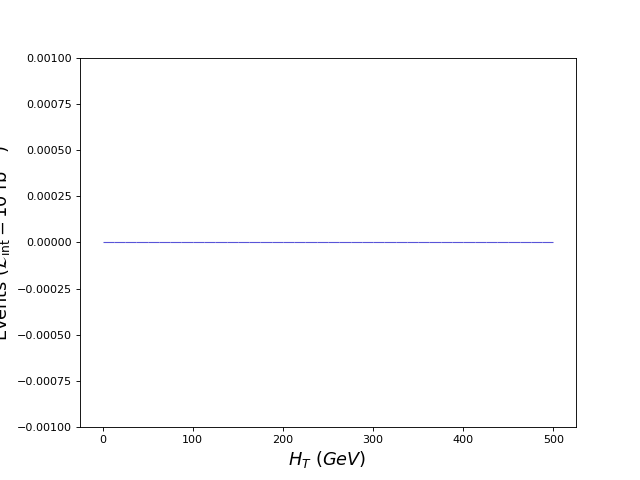
\includegraphics[scale=0.45]{selection_0.png}\\
\caption{   }
  \end{center}
\end{figure}
      \newpage
\subsection{ Histogram 2}

\textbf{* Plot: MET}\\
   \begin{table}[H]
  \begin{center}
    \begin{tabular}{|m{23.0mm}|m{23.0mm}|m{18.0mm}|m{19.0mm}|m{19.0mm}|m{19.0mm}|m{19.0mm}|}
      \hline
      {\cellcolor{yellow}         Dataset}& {\cellcolor{yellow}         Integral}& {\cellcolor{yellow}         Entries per event}& {\cellcolor{yellow}         Mean}& {\cellcolor{yellow}         RMS}& {\cellcolor{yellow}         \% underflow}& {\cellcolor{yellow}         \% overflow}\\
      \hline
      {\cellcolor{white}         unweighted\_events}& {\cellcolor{white}         0.0 +/\-- 0.0}& {\cellcolor{white}         1.0}& {\cellcolor{white}         0.0}& {\cellcolor{white}         0.0}& {\cellcolor{green}         0.0}& {\cellcolor{green}         0.0}\\
\hline
    \end{tabular}
  \end{center}
\end{table}

\begin{table}[H]
  \begin{center}
    \begin{tabular}{|m{140.0mm}|}
      \hline
      {\cellcolor{white}\textcolor{red}{Warnings related to negative event-weights:}}\\
      \hline
      {\cellcolor{white}\textcolor{red}{dataset=unweighted\_events -> bin 0 has a negative content : -1314.515. This value is set to zero}}\\
      \hline
\hline
    \end{tabular}
  \end{center}
\end{table}

\begin{figure}[H]
  \begin{center}
    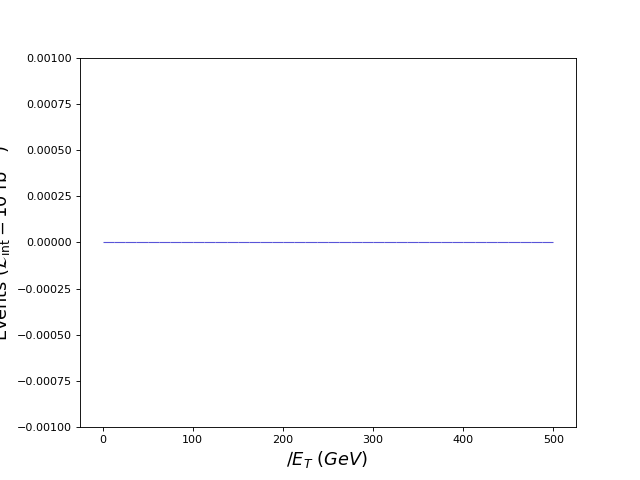
\includegraphics[scale=0.45]{selection_1.png}\\
\caption{   }
  \end{center}
\end{figure}
      \newpage
\subsection{ Histogram 3}

\textbf{* Plot: SQRTS}\\
   \begin{table}[H]
  \begin{center}
    \begin{tabular}{|m{23.0mm}|m{23.0mm}|m{18.0mm}|m{19.0mm}|m{19.0mm}|m{19.0mm}|m{19.0mm}|}
      \hline
      {\cellcolor{yellow}         Dataset}& {\cellcolor{yellow}         Integral}& {\cellcolor{yellow}         Entries per event}& {\cellcolor{yellow}         Mean}& {\cellcolor{yellow}         RMS}& {\cellcolor{yellow}         \% underflow}& {\cellcolor{yellow}         \% overflow}\\
      \hline
      {\cellcolor{white}         unweighted\_events}& {\cellcolor{white}         0.0 +/\-- 0.0}& {\cellcolor{white}         1.0}& {\cellcolor{white}         0.0}& {\cellcolor{white}         0.0}& {\cellcolor{green}         0.0}& {\cellcolor{green}         0.0}\\
\hline
    \end{tabular}
  \end{center}
\end{table}

\begin{table}[H]
  \begin{center}
    \begin{tabular}{|m{140.0mm}|}
      \hline
      {\cellcolor{white}\textcolor{red}{Warnings related to negative event-weights:}}\\
      \hline
      {\cellcolor{white}\textcolor{red}{dataset=unweighted\_events -> bin 27 has a negative content : -8.018543. This value is set to zero}}\\
      \hline
      {\cellcolor{white}\textcolor{red}{dataset=unweighted\_events -> bin 28 has a negative content : -36.67498. This value is set to zero}}\\
      \hline
      {\cellcolor{white}\textcolor{red}{dataset=unweighted\_events -> bin 29 has a negative content : -47.32255. This value is set to zero}}\\
      \hline
      {\cellcolor{white}\textcolor{red}{dataset=unweighted\_events -> bin 30 has a negative content : -47.32255. This value is set to zero}}\\
      \hline
      {\cellcolor{white}\textcolor{red}{dataset=unweighted\_events -> bin 31 has a negative content : -53.50077. This value is set to zero}}\\
      \hline
      {\cellcolor{white}\textcolor{red}{dataset=unweighted\_events -> bin 32 has a negative content : -50.08303. This value is set to zero}}\\
      \hline
      {\cellcolor{white}\textcolor{red}{dataset=unweighted\_events -> bin 33 has a negative content : -52.84352. This value is set to zero}}\\
      \hline
      {\cellcolor{white}\textcolor{red}{dataset=unweighted\_events -> bin 34 has a negative content : -48.11126. This value is set to zero}}\\
      \hline
      {\cellcolor{white}\textcolor{red}{dataset=unweighted\_events -> bin 35 has a negative content : -44.03626. This value is set to zero}}\\
      \hline
      {\cellcolor{white}\textcolor{red}{dataset=unweighted\_events -> bin 36 has a negative content : -44.16771. This value is set to zero}}\\
      \hline
      {\cellcolor{white}\textcolor{red}{dataset=unweighted\_events -> bin 37 has a negative content : -42.5903. This value is set to zero}}\\
      \hline
      {\cellcolor{white}\textcolor{red}{dataset=unweighted\_events -> bin 38 has a negative content : -40.88143. This value is set to zero}}\\
      \hline
      {\cellcolor{white}\textcolor{red}{dataset=unweighted\_events -> bin 39 has a negative content : -38.5153. This value is set to zero}}\\
      \hline
\hline
    \end{tabular}
  \end{center}
\end{table}

\begin{figure}[H]
  \begin{center}
    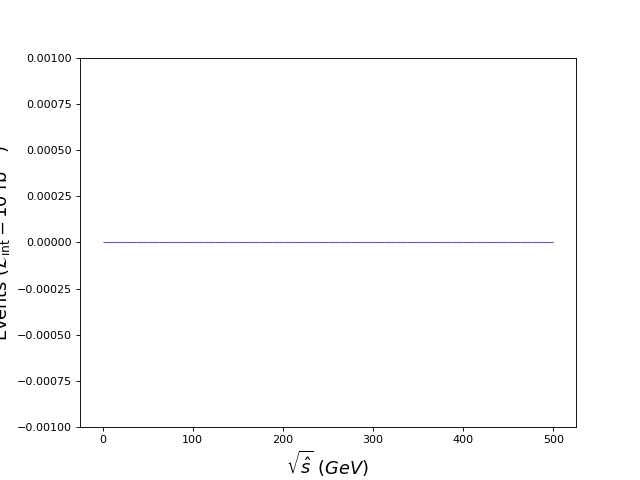
\includegraphics[scale=0.45]{selection_2.png}\\
\caption{   }
  \end{center}
\end{figure}
      \newpage
\subsection{ Histogram 4}

\textbf{* Plot: PT ( t~[1] ) }\\
   \begin{table}[H]
  \begin{center}
    \begin{tabular}{|m{23.0mm}|m{23.0mm}|m{18.0mm}|m{19.0mm}|m{19.0mm}|m{19.0mm}|m{19.0mm}|}
      \hline
      {\cellcolor{yellow}         Dataset}& {\cellcolor{yellow}         Integral}& {\cellcolor{yellow}         Entries per event}& {\cellcolor{yellow}         Mean}& {\cellcolor{yellow}         RMS}& {\cellcolor{yellow}         \% underflow}& {\cellcolor{yellow}         \% overflow}\\
      \hline
      {\cellcolor{white}         unweighted\_events}& {\cellcolor{white}         0.0 +/\-- 0.0}& {\cellcolor{white}         1.0}& {\cellcolor{white}         0.0}& {\cellcolor{white}         0.0}& {\cellcolor{green}         0.0}& {\cellcolor{green}         0.0}\\
\hline
    \end{tabular}
  \end{center}
\end{table}

\begin{table}[H]
  \begin{center}
    \begin{tabular}{|m{140.0mm}|}
      \hline
      {\cellcolor{white}\textcolor{red}{Warnings related to negative event-weights:}}\\
      \hline
      {\cellcolor{white}\textcolor{red}{dataset=unweighted\_events -> bin 0 has a negative content : -14.98547. This value is set to zero}}\\
      \hline
      {\cellcolor{white}\textcolor{red}{dataset=unweighted\_events -> bin 1 has a negative content : -39.82981. This value is set to zero}}\\
      \hline
      {\cellcolor{white}\textcolor{red}{dataset=unweighted\_events -> bin 2 has a negative content : -61.38787. This value is set to zero}}\\
      \hline
      {\cellcolor{white}\textcolor{red}{dataset=unweighted\_events -> bin 3 has a negative content : -79.39673. This value is set to zero}}\\
      \hline
      {\cellcolor{white}\textcolor{red}{dataset=unweighted\_events -> bin 4 has a negative content : -98.983. This value is set to zero}}\\
      \hline
      {\cellcolor{white}\textcolor{red}{dataset=unweighted\_events -> bin 5 has a negative content : -97.27413. This value is set to zero}}\\
      \hline
      {\cellcolor{white}\textcolor{red}{dataset=unweighted\_events -> bin 6 has a negative content : -91.22736. This value is set to zero}}\\
      \hline
      {\cellcolor{white}\textcolor{red}{dataset=unweighted\_events -> bin 7 has a negative content : -93.46204. This value is set to zero}}\\
      \hline
      {\cellcolor{white}\textcolor{red}{dataset=unweighted\_events -> bin 8 has a negative content : -89.25559. This value is set to zero}}\\
      \hline
      {\cellcolor{white}\textcolor{red}{dataset=unweighted\_events -> bin 9 has a negative content : -71.50963. This value is set to zero}}\\
      \hline
      {\cellcolor{white}\textcolor{red}{dataset=unweighted\_events -> bin 10 has a negative content : -65.72577. This value is set to zero}}\\
      \hline
      {\cellcolor{white}\textcolor{red}{dataset=unweighted\_events -> bin 11 has a negative content : -65.06851. This value is set to zero}}\\
      \hline
      {\cellcolor{white}\textcolor{red}{dataset=unweighted\_events -> bin 12 has a negative content : -55.07819. This value is set to zero}}\\
      \hline
      {\cellcolor{white}\textcolor{red}{dataset=unweighted\_events -> bin 13 has a negative content : -44.69352. This value is set to zero}}\\
      \hline
      {\cellcolor{white}\textcolor{red}{dataset=unweighted\_events -> bin 14 has a negative content : -41.14433. This value is set to zero}}\\
      \hline
      {\cellcolor{white}\textcolor{red}{dataset=unweighted\_events -> bin 15 has a negative content : -39.56691. This value is set to zero}}\\
      \hline
      {\cellcolor{white}\textcolor{red}{dataset=unweighted\_events -> bin 16 has a negative content : -32.73143. This value is set to zero}}\\
      \hline
      {\cellcolor{white}\textcolor{red}{dataset=unweighted\_events -> bin 17 has a negative content : -24.18708. This value is set to zero}}\\
      \hline
      {\cellcolor{white}\textcolor{red}{dataset=unweighted\_events -> bin 18 has a negative content : -22.87257. This value is set to zero}}\\
      \hline
      {\cellcolor{white}\textcolor{red}{dataset=unweighted\_events -> bin 19 has a negative content : -21.29515. This value is set to zero}}\\
      \hline
      {\cellcolor{white}\textcolor{red}{dataset=unweighted\_events -> bin 20 has a negative content : -21.29515. This value is set to zero}}\\
      \hline
      {\cellcolor{white}\textcolor{red}{dataset=unweighted\_events -> bin 21 has a negative content : -11.30483. This value is set to zero}}\\
      \hline
      {\cellcolor{white}\textcolor{red}{dataset=unweighted\_events -> bin 22 has a negative content : -14.32822. This value is set to zero}}\\
      \hline
      {\cellcolor{white}\textcolor{red}{dataset=unweighted\_events -> bin 23 has a negative content : -11.04193. This value is set to zero}}\\
      \hline
      {\cellcolor{white}\textcolor{red}{dataset=unweighted\_events -> bin 24 has a negative content : -13.14515. This value is set to zero}}\\
      \hline
      {\cellcolor{white}\textcolor{red}{dataset=unweighted\_events -> bin 25 has a negative content : -10.51612. This value is set to zero}}\\
      \hline
      {\cellcolor{white}\textcolor{red}{dataset=unweighted\_events -> bin 26 has a negative content : -8.938704. This value is set to zero}}\\
      \hline
      {\cellcolor{white}\textcolor{red}{dataset=unweighted\_events -> bin 27 has a negative content : -8.412898. This value is set to zero}}\\
      \hline
      {\cellcolor{white}\textcolor{red}{dataset=unweighted\_events -> bin 28 has a negative content : -4.863707. This value is set to zero}}\\
      \hline
      {\cellcolor{white}\textcolor{red}{dataset=unweighted\_events -> bin 29 has a negative content : -6.441125. This value is set to zero}}\\
      \hline
      {\cellcolor{white}\textcolor{red}{dataset=unweighted\_events -> bin 30 has a negative content : -6.309674. This value is set to zero}}\\
      \hline
      {\cellcolor{white}\textcolor{red}{dataset=unweighted\_events -> bin 31 has a negative content : -5.389513. This value is set to zero}}\\
      \hline
      {\cellcolor{white}\textcolor{red}{dataset=unweighted\_events -> bin 32 has a negative content : -4.863707. This value is set to zero}}\\
      \hline
      {\cellcolor{white}\textcolor{red}{dataset=unweighted\_events -> bin 33 has a negative content : -4.337901. This value is set to zero}}\\
      \hline
      {\cellcolor{white}\textcolor{red}{dataset=unweighted\_events -> bin 34 has a negative content : -3.286288. This value is set to zero}}\\
      \hline
      {\cellcolor{white}\textcolor{red}{dataset=unweighted\_events -> bin 35 has a negative content : -1.971773. This value is set to zero}}\\
      \hline
      {\cellcolor{white}\textcolor{red}{dataset=unweighted\_events -> bin 36 has a negative content : -2.760482. This value is set to zero}}\\
      \hline
      {\cellcolor{white}\textcolor{red}{dataset=unweighted\_events -> bin 37 has a negative content : -3.286288. This value is set to zero}}\\
      \hline
      {\cellcolor{white}\textcolor{red}{dataset=unweighted\_events -> bin 38 has a negative content : -0.7887092. This value is set to zero}}\\
      \hline
      {\cellcolor{white}\textcolor{red}{dataset=unweighted\_events -> bin 39 has a negative content : -1.971773. This value is set to zero}}\\
      \hline
\hline
    \end{tabular}
  \end{center}
\end{table}

\begin{figure}[H]
  \begin{center}
    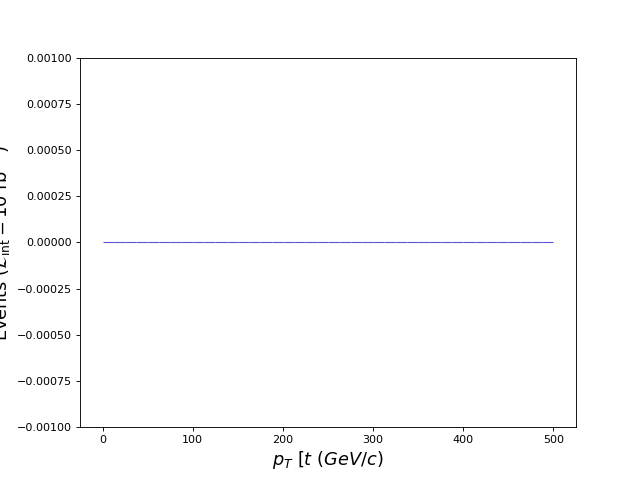
\includegraphics[scale=0.45]{selection_3.png}\\
\caption{   }
  \end{center}
\end{figure}
      \newpage
\subsection{ Histogram 5}

\textbf{* Plot: ETA ( t~[1] ) }\\
   \begin{table}[H]
  \begin{center}
    \begin{tabular}{|m{23.0mm}|m{23.0mm}|m{18.0mm}|m{19.0mm}|m{19.0mm}|m{19.0mm}|m{19.0mm}|}
      \hline
      {\cellcolor{yellow}         Dataset}& {\cellcolor{yellow}         Integral}& {\cellcolor{yellow}         Entries per event}& {\cellcolor{yellow}         Mean}& {\cellcolor{yellow}         RMS}& {\cellcolor{yellow}         \% underflow}& {\cellcolor{yellow}         \% overflow}\\
      \hline
      {\cellcolor{white}         unweighted\_events}& {\cellcolor{white}         0.0 +/\-- 0.0}& {\cellcolor{white}         1.0}& {\cellcolor{white}         0.0}& {\cellcolor{white}         0.0}& {\cellcolor{green}         0.0}& {\cellcolor{green}         0.0}\\
\hline
    \end{tabular}
  \end{center}
\end{table}

\begin{table}[H]
  \begin{center}
    \begin{tabular}{|m{140.0mm}|}
      \hline
      {\cellcolor{white}\textcolor{red}{Warnings related to negative event-weights:}}\\
      \hline
      {\cellcolor{white}\textcolor{red}{dataset=unweighted\_events -> bin 7 has a negative content : -0.1314515. This value is set to zero}}\\
      \hline
      {\cellcolor{white}\textcolor{red}{dataset=unweighted\_events -> bin 8 has a negative content : -0.6572577. This value is set to zero}}\\
      \hline
      {\cellcolor{white}\textcolor{red}{dataset=unweighted\_events -> bin 9 has a negative content : -1.314515. This value is set to zero}}\\
      \hline
      {\cellcolor{white}\textcolor{red}{dataset=unweighted\_events -> bin 10 has a negative content : -3.41774. This value is set to zero}}\\
      \hline
      {\cellcolor{white}\textcolor{red}{dataset=unweighted\_events -> bin 11 has a negative content : -7.098383. This value is set to zero}}\\
      \hline
      {\cellcolor{white}\textcolor{red}{dataset=unweighted\_events -> bin 12 has a negative content : -19.58628. This value is set to zero}}\\
      \hline
      {\cellcolor{white}\textcolor{red}{dataset=unweighted\_events -> bin 13 has a negative content : -40.61852. This value is set to zero}}\\
      \hline
      {\cellcolor{white}\textcolor{red}{dataset=unweighted\_events -> bin 14 has a negative content : -57.18142. This value is set to zero}}\\
      \hline
      {\cellcolor{white}\textcolor{red}{dataset=unweighted\_events -> bin 15 has a negative content : -86.10075. This value is set to zero}}\\
      \hline
      {\cellcolor{white}\textcolor{red}{dataset=unweighted\_events -> bin 16 has a negative content : -103.3209. This value is set to zero}}\\
      \hline
      {\cellcolor{white}\textcolor{red}{dataset=unweighted\_events -> bin 17 has a negative content : -117.912. This value is set to zero}}\\
      \hline
      {\cellcolor{white}\textcolor{red}{dataset=unweighted\_events -> bin 18 has a negative content : -110.0249. This value is set to zero}}\\
      \hline
      {\cellcolor{white}\textcolor{red}{dataset=unweighted\_events -> bin 19 has a negative content : -113.0483. This value is set to zero}}\\
      \hline
      {\cellcolor{white}\textcolor{red}{dataset=unweighted\_events -> bin 20 has a negative content : -106.0814. This value is set to zero}}\\
      \hline
      {\cellcolor{white}\textcolor{red}{dataset=unweighted\_events -> bin 21 has a negative content : -111.4709. This value is set to zero}}\\
      \hline
      {\cellcolor{white}\textcolor{red}{dataset=unweighted\_events -> bin 22 has a negative content : -112.7854. This value is set to zero}}\\
      \hline
      {\cellcolor{white}\textcolor{red}{dataset=unweighted\_events -> bin 23 has a negative content : -111.7338. This value is set to zero}}\\
      \hline
      {\cellcolor{white}\textcolor{red}{dataset=unweighted\_events -> bin 24 has a negative content : -86.23221. This value is set to zero}}\\
      \hline
      {\cellcolor{white}\textcolor{red}{dataset=unweighted\_events -> bin 25 has a negative content : -59.28464. This value is set to zero}}\\
      \hline
      {\cellcolor{white}\textcolor{red}{dataset=unweighted\_events -> bin 26 has a negative content : -35.22901. This value is set to zero}}\\
      \hline
      {\cellcolor{white}\textcolor{red}{dataset=unweighted\_events -> bin 27 has a negative content : -17.61451. This value is set to zero}}\\
      \hline
      {\cellcolor{white}\textcolor{red}{dataset=unweighted\_events -> bin 28 has a negative content : -8.018543. This value is set to zero}}\\
      \hline
      {\cellcolor{white}\textcolor{red}{dataset=unweighted\_events -> bin 29 has a negative content : -4.206449. This value is set to zero}}\\
      \hline
      {\cellcolor{white}\textcolor{red}{dataset=unweighted\_events -> bin 30 has a negative content : -0.5258061. This value is set to zero}}\\
      \hline
      {\cellcolor{white}\textcolor{red}{dataset=unweighted\_events -> bin 31 has a negative content : -0.5258061. This value is set to zero}}\\
      \hline
      {\cellcolor{white}\textcolor{red}{dataset=unweighted\_events -> bin 32 has a negative content : -0.2629031. This value is set to zero}}\\
      \hline
      {\cellcolor{white}\textcolor{red}{dataset=unweighted\_events -> bin 33 has a negative content : -0.1314515. This value is set to zero}}\\
      \hline
\hline
    \end{tabular}
  \end{center}
\end{table}

\begin{figure}[H]
  \begin{center}
    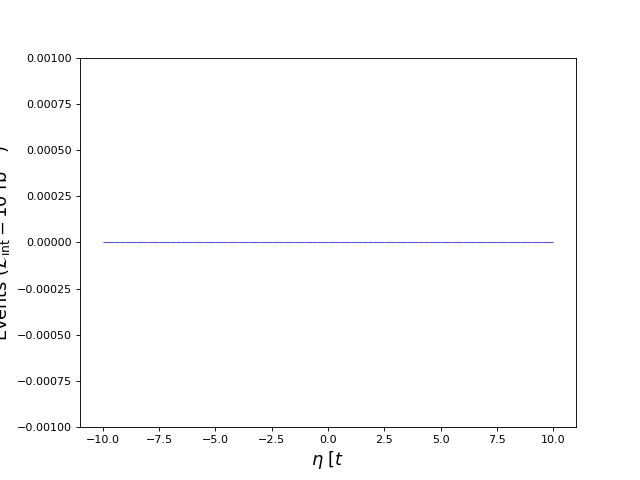
\includegraphics[scale=0.45]{selection_4.png}\\
\caption{   }
  \end{center}
\end{figure}
      \newpage
\subsection{ Histogram 6}

\textbf{* Plot: PT ( t[1] ) }\\
   \begin{table}[H]
  \begin{center}
    \begin{tabular}{|m{23.0mm}|m{23.0mm}|m{18.0mm}|m{19.0mm}|m{19.0mm}|m{19.0mm}|m{19.0mm}|}
      \hline
      {\cellcolor{yellow}         Dataset}& {\cellcolor{yellow}         Integral}& {\cellcolor{yellow}         Entries per event}& {\cellcolor{yellow}         Mean}& {\cellcolor{yellow}         RMS}& {\cellcolor{yellow}         \% underflow}& {\cellcolor{yellow}         \% overflow}\\
      \hline
      {\cellcolor{white}         unweighted\_events}& {\cellcolor{white}         0.0 +/\-- 0.0}& {\cellcolor{white}         1.0}& {\cellcolor{white}         0.0}& {\cellcolor{white}         0.0}& {\cellcolor{green}         0.0}& {\cellcolor{green}         0.0}\\
\hline
    \end{tabular}
  \end{center}
\end{table}

\begin{table}[H]
  \begin{center}
    \begin{tabular}{|m{140.0mm}|}
      \hline
      {\cellcolor{white}\textcolor{red}{Warnings related to negative event-weights:}}\\
      \hline
      {\cellcolor{white}\textcolor{red}{dataset=unweighted\_events -> bin 0 has a negative content : -14.98547. This value is set to zero}}\\
      \hline
      {\cellcolor{white}\textcolor{red}{dataset=unweighted\_events -> bin 1 has a negative content : -39.82981. This value is set to zero}}\\
      \hline
      {\cellcolor{white}\textcolor{red}{dataset=unweighted\_events -> bin 2 has a negative content : -61.38787. This value is set to zero}}\\
      \hline
      {\cellcolor{white}\textcolor{red}{dataset=unweighted\_events -> bin 3 has a negative content : -79.39673. This value is set to zero}}\\
      \hline
      {\cellcolor{white}\textcolor{red}{dataset=unweighted\_events -> bin 4 has a negative content : -98.983. This value is set to zero}}\\
      \hline
      {\cellcolor{white}\textcolor{red}{dataset=unweighted\_events -> bin 5 has a negative content : -97.27413. This value is set to zero}}\\
      \hline
      {\cellcolor{white}\textcolor{red}{dataset=unweighted\_events -> bin 6 has a negative content : -91.22736. This value is set to zero}}\\
      \hline
      {\cellcolor{white}\textcolor{red}{dataset=unweighted\_events -> bin 7 has a negative content : -93.46204. This value is set to zero}}\\
      \hline
      {\cellcolor{white}\textcolor{red}{dataset=unweighted\_events -> bin 8 has a negative content : -89.25559. This value is set to zero}}\\
      \hline
      {\cellcolor{white}\textcolor{red}{dataset=unweighted\_events -> bin 9 has a negative content : -71.50963. This value is set to zero}}\\
      \hline
      {\cellcolor{white}\textcolor{red}{dataset=unweighted\_events -> bin 10 has a negative content : -65.72577. This value is set to zero}}\\
      \hline
      {\cellcolor{white}\textcolor{red}{dataset=unweighted\_events -> bin 11 has a negative content : -65.06851. This value is set to zero}}\\
      \hline
      {\cellcolor{white}\textcolor{red}{dataset=unweighted\_events -> bin 12 has a negative content : -55.07819. This value is set to zero}}\\
      \hline
      {\cellcolor{white}\textcolor{red}{dataset=unweighted\_events -> bin 13 has a negative content : -44.69352. This value is set to zero}}\\
      \hline
      {\cellcolor{white}\textcolor{red}{dataset=unweighted\_events -> bin 14 has a negative content : -41.14433. This value is set to zero}}\\
      \hline
      {\cellcolor{white}\textcolor{red}{dataset=unweighted\_events -> bin 15 has a negative content : -39.56691. This value is set to zero}}\\
      \hline
      {\cellcolor{white}\textcolor{red}{dataset=unweighted\_events -> bin 16 has a negative content : -32.73143. This value is set to zero}}\\
      \hline
      {\cellcolor{white}\textcolor{red}{dataset=unweighted\_events -> bin 17 has a negative content : -24.18708. This value is set to zero}}\\
      \hline
      {\cellcolor{white}\textcolor{red}{dataset=unweighted\_events -> bin 18 has a negative content : -22.87257. This value is set to zero}}\\
      \hline
      {\cellcolor{white}\textcolor{red}{dataset=unweighted\_events -> bin 19 has a negative content : -21.29515. This value is set to zero}}\\
      \hline
      {\cellcolor{white}\textcolor{red}{dataset=unweighted\_events -> bin 20 has a negative content : -21.29515. This value is set to zero}}\\
      \hline
      {\cellcolor{white}\textcolor{red}{dataset=unweighted\_events -> bin 21 has a negative content : -11.30483. This value is set to zero}}\\
      \hline
      {\cellcolor{white}\textcolor{red}{dataset=unweighted\_events -> bin 22 has a negative content : -14.32822. This value is set to zero}}\\
      \hline
      {\cellcolor{white}\textcolor{red}{dataset=unweighted\_events -> bin 23 has a negative content : -11.04193. This value is set to zero}}\\
      \hline
      {\cellcolor{white}\textcolor{red}{dataset=unweighted\_events -> bin 24 has a negative content : -13.14515. This value is set to zero}}\\
      \hline
      {\cellcolor{white}\textcolor{red}{dataset=unweighted\_events -> bin 25 has a negative content : -10.51612. This value is set to zero}}\\
      \hline
      {\cellcolor{white}\textcolor{red}{dataset=unweighted\_events -> bin 26 has a negative content : -8.938704. This value is set to zero}}\\
      \hline
      {\cellcolor{white}\textcolor{red}{dataset=unweighted\_events -> bin 27 has a negative content : -8.412898. This value is set to zero}}\\
      \hline
      {\cellcolor{white}\textcolor{red}{dataset=unweighted\_events -> bin 28 has a negative content : -4.863707. This value is set to zero}}\\
      \hline
      {\cellcolor{white}\textcolor{red}{dataset=unweighted\_events -> bin 29 has a negative content : -6.441125. This value is set to zero}}\\
      \hline
      {\cellcolor{white}\textcolor{red}{dataset=unweighted\_events -> bin 30 has a negative content : -6.309674. This value is set to zero}}\\
      \hline
      {\cellcolor{white}\textcolor{red}{dataset=unweighted\_events -> bin 31 has a negative content : -5.389513. This value is set to zero}}\\
      \hline
      {\cellcolor{white}\textcolor{red}{dataset=unweighted\_events -> bin 32 has a negative content : -4.863707. This value is set to zero}}\\
      \hline
      {\cellcolor{white}\textcolor{red}{dataset=unweighted\_events -> bin 33 has a negative content : -4.337901. This value is set to zero}}\\
      \hline
      {\cellcolor{white}\textcolor{red}{dataset=unweighted\_events -> bin 34 has a negative content : -3.286288. This value is set to zero}}\\
      \hline
      {\cellcolor{white}\textcolor{red}{dataset=unweighted\_events -> bin 35 has a negative content : -1.971773. This value is set to zero}}\\
      \hline
      {\cellcolor{white}\textcolor{red}{dataset=unweighted\_events -> bin 36 has a negative content : -2.760482. This value is set to zero}}\\
      \hline
      {\cellcolor{white}\textcolor{red}{dataset=unweighted\_events -> bin 37 has a negative content : -3.286288. This value is set to zero}}\\
      \hline
      {\cellcolor{white}\textcolor{red}{dataset=unweighted\_events -> bin 38 has a negative content : -0.7887092. This value is set to zero}}\\
      \hline
      {\cellcolor{white}\textcolor{red}{dataset=unweighted\_events -> bin 39 has a negative content : -1.971773. This value is set to zero}}\\
      \hline
\hline
    \end{tabular}
  \end{center}
\end{table}

\begin{figure}[H]
  \begin{center}
    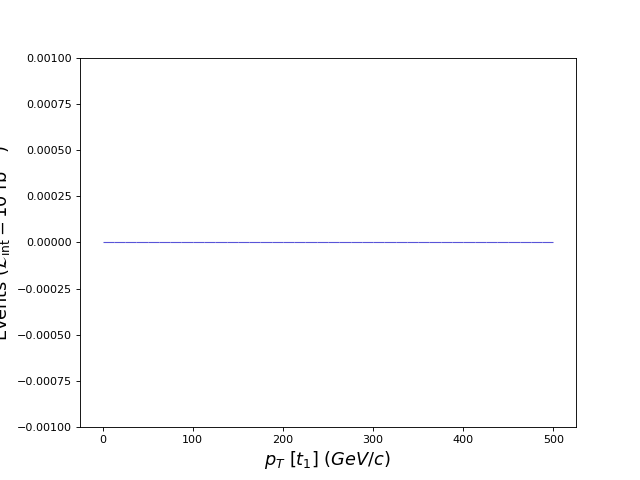
\includegraphics[scale=0.45]{selection_5.png}\\
\caption{   }
  \end{center}
\end{figure}
      \newpage
\subsection{ Histogram 7}

\textbf{* Plot: ETA ( t[1] ) }\\
   \begin{table}[H]
  \begin{center}
    \begin{tabular}{|m{23.0mm}|m{23.0mm}|m{18.0mm}|m{19.0mm}|m{19.0mm}|m{19.0mm}|m{19.0mm}|}
      \hline
      {\cellcolor{yellow}         Dataset}& {\cellcolor{yellow}         Integral}& {\cellcolor{yellow}         Entries per event}& {\cellcolor{yellow}         Mean}& {\cellcolor{yellow}         RMS}& {\cellcolor{yellow}         \% underflow}& {\cellcolor{yellow}         \% overflow}\\
      \hline
      {\cellcolor{white}         unweighted\_events}& {\cellcolor{white}         0.0 +/\-- 0.0}& {\cellcolor{white}         1.0}& {\cellcolor{white}         0.0}& {\cellcolor{white}         0.0}& {\cellcolor{green}         0.0}& {\cellcolor{green}         0.0}\\
\hline
    \end{tabular}
  \end{center}
\end{table}

\begin{table}[H]
  \begin{center}
    \begin{tabular}{|m{140.0mm}|}
      \hline
      {\cellcolor{white}\textcolor{red}{Warnings related to negative event-weights:}}\\
      \hline
      {\cellcolor{white}\textcolor{red}{dataset=unweighted\_events -> bin 6 has a negative content : -0.3943546. This value is set to zero}}\\
      \hline
      {\cellcolor{white}\textcolor{red}{dataset=unweighted\_events -> bin 7 has a negative content : -0.1314515. This value is set to zero}}\\
      \hline
      {\cellcolor{white}\textcolor{red}{dataset=unweighted\_events -> bin 8 has a negative content : -0.5258061. This value is set to zero}}\\
      \hline
      {\cellcolor{white}\textcolor{red}{dataset=unweighted\_events -> bin 9 has a negative content : -1.314515. This value is set to zero}}\\
      \hline
      {\cellcolor{white}\textcolor{red}{dataset=unweighted\_events -> bin 10 has a negative content : -3.943546. This value is set to zero}}\\
      \hline
      {\cellcolor{white}\textcolor{red}{dataset=unweighted\_events -> bin 11 has a negative content : -8.807253. This value is set to zero}}\\
      \hline
      {\cellcolor{white}\textcolor{red}{dataset=unweighted\_events -> bin 12 has a negative content : -17.61451. This value is set to zero}}\\
      \hline
      {\cellcolor{white}\textcolor{red}{dataset=unweighted\_events -> bin 13 has a negative content : -35.09756. This value is set to zero}}\\
      \hline
      {\cellcolor{white}\textcolor{red}{dataset=unweighted\_events -> bin 14 has a negative content : -60.86206. This value is set to zero}}\\
      \hline
      {\cellcolor{white}\textcolor{red}{dataset=unweighted\_events -> bin 15 has a negative content : -86.88946. This value is set to zero}}\\
      \hline
      {\cellcolor{white}\textcolor{red}{dataset=unweighted\_events -> bin 16 has a negative content : -108.1846. This value is set to zero}}\\
      \hline
      {\cellcolor{white}\textcolor{red}{dataset=unweighted\_events -> bin 17 has a negative content : -114.4943. This value is set to zero}}\\
      \hline
      {\cellcolor{white}\textcolor{red}{dataset=unweighted\_events -> bin 18 has a negative content : -116.4661. This value is set to zero}}\\
      \hline
      {\cellcolor{white}\textcolor{red}{dataset=unweighted\_events -> bin 19 has a negative content : -101.2177. This value is set to zero}}\\
      \hline
      {\cellcolor{white}\textcolor{red}{dataset=unweighted\_events -> bin 20 has a negative content : -111.8653. This value is set to zero}}\\
      \hline
      {\cellcolor{white}\textcolor{red}{dataset=unweighted\_events -> bin 21 has a negative content : -109.762. This value is set to zero}}\\
      \hline
      {\cellcolor{white}\textcolor{red}{dataset=unweighted\_events -> bin 22 has a negative content : -113.7056. This value is set to zero}}\\
      \hline
      {\cellcolor{white}\textcolor{red}{dataset=unweighted\_events -> bin 23 has a negative content : -108.4475. This value is set to zero}}\\
      \hline
      {\cellcolor{white}\textcolor{red}{dataset=unweighted\_events -> bin 24 has a negative content : -85.04914. This value is set to zero}}\\
      \hline
      {\cellcolor{white}\textcolor{red}{dataset=unweighted\_events -> bin 25 has a negative content : -63.62254. This value is set to zero}}\\
      \hline
      {\cellcolor{white}\textcolor{red}{dataset=unweighted\_events -> bin 26 has a negative content : -36.54353. This value is set to zero}}\\
      \hline
      {\cellcolor{white}\textcolor{red}{dataset=unweighted\_events -> bin 27 has a negative content : -18.40321. This value is set to zero}}\\
      \hline
      {\cellcolor{white}\textcolor{red}{dataset=unweighted\_events -> bin 28 has a negative content : -7.229834. This value is set to zero}}\\
      \hline
      {\cellcolor{white}\textcolor{red}{dataset=unweighted\_events -> bin 29 has a negative content : -2.497579. This value is set to zero}}\\
      \hline
      {\cellcolor{white}\textcolor{red}{dataset=unweighted\_events -> bin 30 has a negative content : -1.183064. This value is set to zero}}\\
      \hline
      {\cellcolor{white}\textcolor{red}{dataset=unweighted\_events -> bin 31 has a negative content : -0.1314515. This value is set to zero}}\\
      \hline
      {\cellcolor{white}\textcolor{red}{dataset=unweighted\_events -> bin 34 has a negative content : -0.1314515. This value is set to zero}}\\
      \hline
\hline
    \end{tabular}
  \end{center}
\end{table}

\begin{figure}[H]
  \begin{center}
    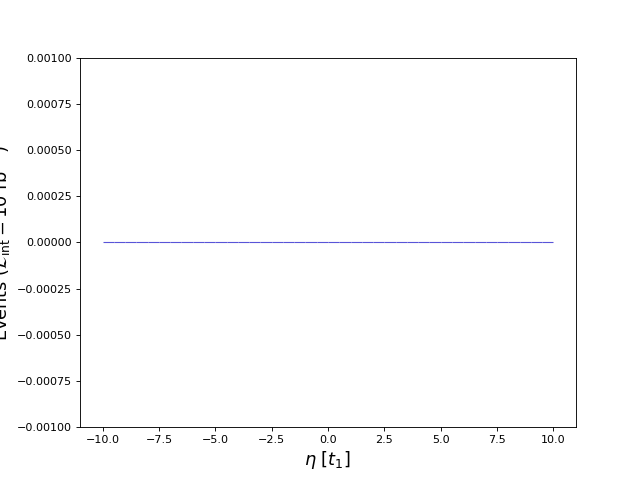
\includegraphics[scale=0.45]{selection_6.png}\\
\caption{   }
  \end{center}
\end{figure}
      \newpage
\subsection{ Histogram 8}

\textbf{* Plot: M ( t[1] t~[1] ) }\\
   \begin{table}[H]
  \begin{center}
    \begin{tabular}{|m{23.0mm}|m{23.0mm}|m{18.0mm}|m{19.0mm}|m{19.0mm}|m{19.0mm}|m{19.0mm}|}
      \hline
      {\cellcolor{yellow}         Dataset}& {\cellcolor{yellow}         Integral}& {\cellcolor{yellow}         Entries per event}& {\cellcolor{yellow}         Mean}& {\cellcolor{yellow}         RMS}& {\cellcolor{yellow}         \% underflow}& {\cellcolor{yellow}         \% overflow}\\
      \hline
      {\cellcolor{white}         unweighted\_events}& {\cellcolor{white}         0.0 +/\-- 0.0}& {\cellcolor{white}         1.0}& {\cellcolor{white}         0.0}& {\cellcolor{white}         0.0}& {\cellcolor{green}         0.0}& {\cellcolor{green}         0.0}\\
\hline
    \end{tabular}
  \end{center}
\end{table}

\begin{table}[H]
  \begin{center}
    \begin{tabular}{|m{140.0mm}|}
      \hline
      {\cellcolor{white}\textcolor{red}{Warnings related to negative event-weights:}}\\
      \hline
      {\cellcolor{white}\textcolor{red}{dataset=unweighted\_events -> bin 27 has a negative content : -8.018543. This value is set to zero}}\\
      \hline
      {\cellcolor{white}\textcolor{red}{dataset=unweighted\_events -> bin 28 has a negative content : -36.67498. This value is set to zero}}\\
      \hline
      {\cellcolor{white}\textcolor{red}{dataset=unweighted\_events -> bin 29 has a negative content : -47.32255. This value is set to zero}}\\
      \hline
      {\cellcolor{white}\textcolor{red}{dataset=unweighted\_events -> bin 30 has a negative content : -47.32255. This value is set to zero}}\\
      \hline
      {\cellcolor{white}\textcolor{red}{dataset=unweighted\_events -> bin 31 has a negative content : -53.50077. This value is set to zero}}\\
      \hline
      {\cellcolor{white}\textcolor{red}{dataset=unweighted\_events -> bin 32 has a negative content : -50.08303. This value is set to zero}}\\
      \hline
      {\cellcolor{white}\textcolor{red}{dataset=unweighted\_events -> bin 33 has a negative content : -52.84352. This value is set to zero}}\\
      \hline
      {\cellcolor{white}\textcolor{red}{dataset=unweighted\_events -> bin 34 has a negative content : -48.11126. This value is set to zero}}\\
      \hline
      {\cellcolor{white}\textcolor{red}{dataset=unweighted\_events -> bin 35 has a negative content : -44.03626. This value is set to zero}}\\
      \hline
      {\cellcolor{white}\textcolor{red}{dataset=unweighted\_events -> bin 36 has a negative content : -44.16771. This value is set to zero}}\\
      \hline
      {\cellcolor{white}\textcolor{red}{dataset=unweighted\_events -> bin 37 has a negative content : -42.5903. This value is set to zero}}\\
      \hline
      {\cellcolor{white}\textcolor{red}{dataset=unweighted\_events -> bin 38 has a negative content : -40.88143. This value is set to zero}}\\
      \hline
      {\cellcolor{white}\textcolor{red}{dataset=unweighted\_events -> bin 39 has a negative content : -38.5153. This value is set to zero}}\\
      \hline
\hline
    \end{tabular}
  \end{center}
\end{table}

\begin{figure}[H]
  \begin{center}
    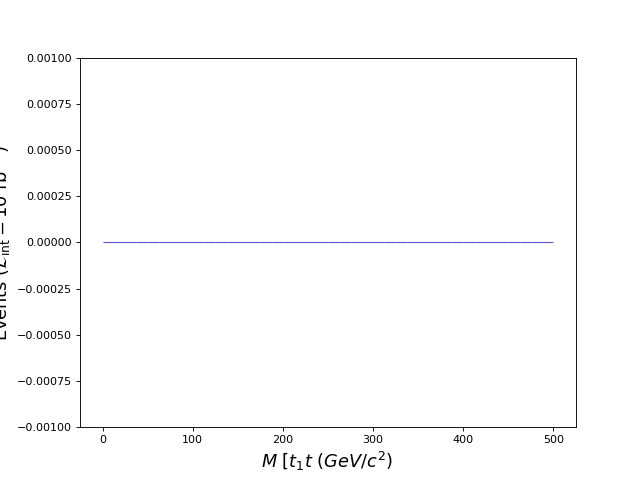
\includegraphics[scale=0.45]{selection_7.png}\\
\caption{   }
  \end{center}
\end{figure}
      \newpage
\subsection{ Histogram 9}

\textbf{* Plot: DELTAR ( t~[1] , t[1] ) }\\
   \begin{table}[H]
  \begin{center}
    \begin{tabular}{|m{23.0mm}|m{23.0mm}|m{18.0mm}|m{19.0mm}|m{19.0mm}|m{19.0mm}|m{19.0mm}|}
      \hline
      {\cellcolor{yellow}         Dataset}& {\cellcolor{yellow}         Integral}& {\cellcolor{yellow}         Entries per event}& {\cellcolor{yellow}         Mean}& {\cellcolor{yellow}         RMS}& {\cellcolor{yellow}         \% underflow}& {\cellcolor{yellow}         \% overflow}\\
      \hline
      {\cellcolor{white}         unweighted\_events}& {\cellcolor{white}         0.0 +/\-- 0.0}& {\cellcolor{white}         1.0}& {\cellcolor{white}         0.0}& {\cellcolor{white}         0.0}& {\cellcolor{green}         0.0}& {\cellcolor{green}         0.0}\\
\hline
    \end{tabular}
  \end{center}
\end{table}

\begin{table}[H]
  \begin{center}
    \begin{tabular}{|m{140.0mm}|}
      \hline
      {\cellcolor{white}\textcolor{red}{Warnings related to negative event-weights:}}\\
      \hline
      {\cellcolor{white}\textcolor{red}{dataset=unweighted\_events -> bin 12 has a negative content : -383.1812. This value is set to zero}}\\
      \hline
      {\cellcolor{white}\textcolor{red}{dataset=unweighted\_events -> bin 13 has a negative content : -282.6208. This value is set to zero}}\\
      \hline
      {\cellcolor{white}\textcolor{red}{dataset=unweighted\_events -> bin 14 has a negative content : -165.7604. This value is set to zero}}\\
      \hline
      {\cellcolor{white}\textcolor{red}{dataset=unweighted\_events -> bin 15 has a negative content : -111.8653. This value is set to zero}}\\
      \hline
      {\cellcolor{white}\textcolor{red}{dataset=unweighted\_events -> bin 16 has a negative content : -84.65479. This value is set to zero}}\\
      \hline
      {\cellcolor{white}\textcolor{red}{dataset=unweighted\_events -> bin 17 has a negative content : -61.51932. This value is set to zero}}\\
      \hline
      {\cellcolor{white}\textcolor{red}{dataset=unweighted\_events -> bin 18 has a negative content : -42.72175. This value is set to zero}}\\
      \hline
      {\cellcolor{white}\textcolor{red}{dataset=unweighted\_events -> bin 19 has a negative content : -36.80643. This value is set to zero}}\\
      \hline
      {\cellcolor{white}\textcolor{red}{dataset=unweighted\_events -> bin 20 has a negative content : -31.02256. This value is set to zero}}\\
      \hline
      {\cellcolor{white}\textcolor{red}{dataset=unweighted\_events -> bin 21 has a negative content : -24.44998. This value is set to zero}}\\
      \hline
      {\cellcolor{white}\textcolor{red}{dataset=unweighted\_events -> bin 22 has a negative content : -19.98063. This value is set to zero}}\\
      \hline
      {\cellcolor{white}\textcolor{red}{dataset=unweighted\_events -> bin 23 has a negative content : -15.37983. This value is set to zero}}\\
      \hline
      {\cellcolor{white}\textcolor{red}{dataset=unweighted\_events -> bin 24 has a negative content : -10.64757. This value is set to zero}}\\
      \hline
      {\cellcolor{white}\textcolor{red}{dataset=unweighted\_events -> bin 25 has a negative content : -7.887092. This value is set to zero}}\\
      \hline
      {\cellcolor{white}\textcolor{red}{dataset=unweighted\_events -> bin 26 has a negative content : -10.38467. This value is set to zero}}\\
      \hline
      {\cellcolor{white}\textcolor{red}{dataset=unweighted\_events -> bin 27 has a negative content : -5.389513. This value is set to zero}}\\
      \hline
      {\cellcolor{white}\textcolor{red}{dataset=unweighted\_events -> bin 28 has a negative content : -4.074997. This value is set to zero}}\\
      \hline
      {\cellcolor{white}\textcolor{red}{dataset=unweighted\_events -> bin 29 has a negative content : -3.549191. This value is set to zero}}\\
      \hline
      {\cellcolor{white}\textcolor{red}{dataset=unweighted\_events -> bin 30 has a negative content : -2.497579. This value is set to zero}}\\
      \hline
      {\cellcolor{white}\textcolor{red}{dataset=unweighted\_events -> bin 31 has a negative content : -2.366128. This value is set to zero}}\\
      \hline
      {\cellcolor{white}\textcolor{red}{dataset=unweighted\_events -> bin 32 has a negative content : -1.70887. This value is set to zero}}\\
      \hline
      {\cellcolor{white}\textcolor{red}{dataset=unweighted\_events -> bin 33 has a negative content : -1.971773. This value is set to zero}}\\
      \hline
      {\cellcolor{white}\textcolor{red}{dataset=unweighted\_events -> bin 34 has a negative content : -0.5258061. This value is set to zero}}\\
      \hline
      {\cellcolor{white}\textcolor{red}{dataset=unweighted\_events -> bin 35 has a negative content : -0.7887092. This value is set to zero}}\\
      \hline
      {\cellcolor{white}\textcolor{red}{dataset=unweighted\_events -> bin 36 has a negative content : -1.183064. This value is set to zero}}\\
      \hline
      {\cellcolor{white}\textcolor{red}{dataset=unweighted\_events -> bin 37 has a negative content : -0.5258061. This value is set to zero}}\\
      \hline
      {\cellcolor{white}\textcolor{red}{dataset=unweighted\_events -> bin 38 has a negative content : -0.1314515. This value is set to zero}}\\
      \hline
      {\cellcolor{white}\textcolor{red}{dataset=unweighted\_events -> bin 39 has a negative content : -0.2629031. This value is set to zero}}\\
      \hline
\hline
    \end{tabular}
  \end{center}
\end{table}

\begin{figure}[H]
  \begin{center}
    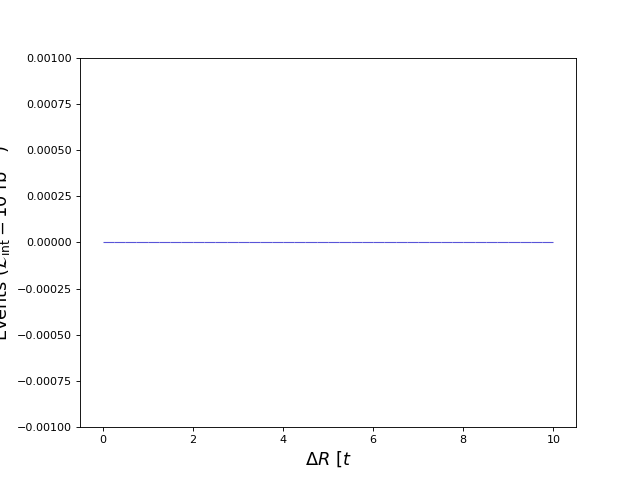
\includegraphics[scale=0.45]{selection_8.png}\\
\caption{   }
  \end{center}
\end{figure}
      \end{document}
